\documentclass{../UTNetLab}

\title{Linux and TCP/IP Networking}
\authorshort{A. Khonsari, A. HajiAliKhamseh'i, M. Borhani, A. Khordadi, S. Kashipazha}
\author{%
    Dr. Ahmad Khonsari\\
    \FR{دکتر احمد خونساری}\\
    \mail{a\_khonsari@ut.ac.ir}
    \end{tabular}\vskip 1em
    \begin{tabular}[t]{c}
    Amir Haji Ali Khamseh'i\\
    \FR{امیر حاجی‌علی‌خمسه‌ء}\\
    \mail{khamse@ut.ac.ir}
    \and
    {Muhammad Borhani}\\
    \FR{محمد برهانی}\\
    \mail{m.borhani@ut.ac.ir}
    \and
    {AmirAhmad Khordadi}\\
    \FR{امیراحمد خردادی}\\
    \mail{a.a.khordadi@ut.ac.ir}
    \and
    {Sina Kashipazha}\\
    \FR{سینا کاشی‌پزها}\\
    \mail{sina\_kashipazha@ut.ac.ir}
    \and
    {Hadi Safari}\\
    \FR{هادی صفری}\\
    \mail{hadi.safari@ut.ac.ir}
    \and
    % {alii}\\
    % \FR{دیگران}\\
    % \mail{info@example.com}
}

\begin{document}
\section*{Systems Configuration}
    Launch GNS3 and make a network as below. You can use \lstinline{ifconfig eth0 192.168.0.1 netmask 255.255.255.0} to set ip.
    \begin{center}
        \begin{minipage}{0.48\textwidth}
            \begin{flushleft}
                \begin{table}[H]
                    \caption{The IP addresses of the hosts}
                    \centering
                    \begin{tabular}{ l l l }
                        \hline \hline
                        Host & IP Address & Subnet Mask \\
                        \hline 
                        h0 (shakti) & 128.238.66.100 & 255.255.255.0 \\
                        h1 (vayu) & 128.238.66.101 & 255.255.255.0 \\
                        h2 (agni) & 128.238.66.102 & 255.255.255.0 \\
                        h3 (apah) & 128.238.66.103 & 255.255.255.0 \\
                        h4 (yachi) & 128.238.66.104 & 255.255.255.0 \\
                        h5 (fenchi) & 128.238.66.105 & 255.255.255.0 \\
                        h6 (kenchi) & 128.238.66.106 & 255.255.255.0 \\
                        h7 (guchi) & 128.238.66.107 & 255.255.255.0 \\
                        \hline \hline
                        \end{tabular}
                \end{table}
            \end{flushleft}
        \end{minipage}
        \begin{minipage}{0.48\textwidth}
            \begin{flushright}
                \begin{figure}[H]
                    \centering
                    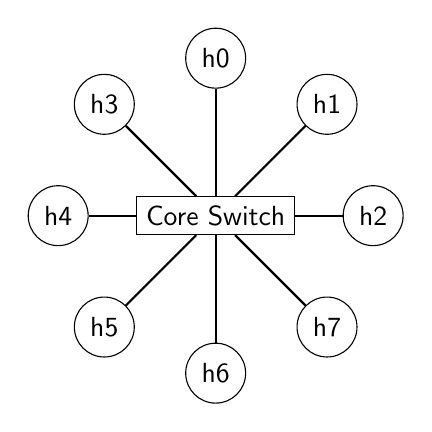
\begin{tikzpicture}[font=\sf]
                        \node[draw] (s) at (0,0){Core Switch};
                        \node[draw,circle] (h0) at (0,2){h0};
                        \node[draw,circle] (h1) at ({sqrt(2)},{sqrt(2)}){h1};
                        \node[draw,circle] (h2) at (2,0){h2};
                        \node[draw,circle] (h3) at (-{sqrt(2)},{sqrt(2)}){h3};
                        \node[draw,circle] (h4) at (-2,0){h4};
                        \node[draw,circle] (h5) at (-{sqrt(2)},-{sqrt(2)}){h5};
                        \node[draw,circle] (h6) at (0,-2){h6};
                        \node[draw,circle] (h7) at ({sqrt(2)},-{sqrt(2)}){h7};
                    
                        \draw[thick] (h0) -- (s);
                        \draw[thick] (h1) -- (s);
                        \draw[thick] (h2) -- (s);
                        \draw[thick] (h3) -- (s);
                        \draw[thick] (h4) -- (s);
                        \draw[thick] (h5) -- (s);
                        \draw[thick] (h6) -- (s);
                        \draw[thick] (h7) -- (s);
                    \end{tikzpicture}
                    \caption{A single segment network}        
                \end{figure}
            \end{flushright}
        \end{minipage}
    \end{center}

\section{Telnet Service}
    Run \lstinline{ps -e} to list the processes running in \textit{h1}.
    After starting a new process by running \lstinline{telnet} in another command window, execute \lstinline{ps -e} again in a third window to see if there is any change in its output.

    Find the process id of the \lstinline{telnet} process you started, by:
    \begin{lstlisting}
ps -e | grep telnet
    \end{lstlisting}
    Then use \lstinline[emph={process-id-of-telnet}]{kill process-id-of-telnet} to terminate the \lstinline{telnet} process.
    
    \subsection*{Report}
    What is Internet Service Daemon (\lstinline{inetd})?

    Is \lstinline{inetd} started in your system?
    Why?

    Is \lstinline{xinetd} started in your system? What is its PID?

\section{Default Network Services}
    Display the file \path{/etc/services} on \textit{h1} screen, using:
    \begin{lstlisting}
more /etc/services
    \end{lstlisting}
    Then in another console, use the redirect operator to redirect the \lstinline{more} output to
    a file using \lstinline{more /etc/services > ser-more}. Compare the file \path{ser-more} with the original \lstinline{more} output in the other command window.

    Copy \path{/etc/services} file to a local file named \path{ser-cp} in your working directory,
    using \lstinline{cp /etc/services ser-cp}. Compare files \path{ser-more} and \path{ser-cp}, using \lstinline{cmp ser-more ser-cp}. Are these two files identical?

    Concatenate these two files using \lstinline{cat ser-more ser-cp > ser-cat}.

    Display the file sizes using \lstinline{ls -l ser*}. Save the output. What are the sizes of files \path{ser-more}, \path{ser-cp}, and \path{ser-cat}?

\section{Network Command Manual}
    Read the \lstinline{man} pages for the following programs:
    \begin{multicols}{3}
        \begin{enumerate}
            \item \lstinline{arp}
            \item \lstinline{arping}
            \item \lstinline{ifconfig}
            \item \lstinline{tcpdump}
            \item \lstinline{ping}
            \item \lstinline{netstat}
            \item \lstinline{route}
            \item \lstinline{wireshark}
            \item \lstinline{iptables}
        \end{enumerate}
    \end{multicols}
    Study the different options associated with each command.
    Throughout this lab you will use these commands rather extensively.
    
    \subsection*{Report}
    Explain the above commands briefly.
    Two or three sentences per command would be adequate.

\section{Packet Capturing}
    In this exercise, we will use \lstinline{tcpdump} to capture a packet containing the link, IP, and TCP headers and use \lstinline{wireshark} to analyze this packet.

    First, run \lstinline{tcpdump -enx -w dump.out} in \textit{h1}.
    You will not see any \lstinline{tcpdump} output, since the \lstinline{-w} option is used to write the output to the \path{dump.out} file.

    Then, you may want to run \lstinline{telnet 10.0.0.2} to generate some TCP traffic.\footnote{Remember to run \lstinline{/etc/init.d/xinetd restart} in \textit{h2} to start telnet server on it.}
    After you login to \textit{h2}, terminate the \lstinline{telnet} session and terminate the \lstinline{tcpdump} program.
    Next, you will use \lstinline{wireshark} to open the packet trace captured by \lstinline{tcpdump} and analyze the captured packets.
    To do this, run \lstinline{wireshark dump.out &}.
    The \lstinline{wireshark} Graphical User Interface (GUI) will pop up and the packets captured by \lstinline{tcpdump} will be displayed.
    Select any one of the packets that contain the link, IP, and TCP headers.
    
    \subsection*{Report}
    What is the value of the \texttt{protocol} field in the IP header of the packet you saved?
    What is the use of the \texttt{protocol} field?

    What is the value of the \texttt{frame type} field in an Ethernet frame carrying an IP datagram?

\section{\texttt{ARPing}}
    This time we will run wireshark to capture an ARP request and an ARP reply in real-time. Simply run \lstinline{wireshark &} in \textit{h1} and select the interface and start capturing.
    If there is no arp requests and replies in the network, generate some using \lstinline{arping 10.0.0.2}.

    Now you should see several ARP replies in the arping output.
    
    \subsection*{Report}
    What is the value of the \texttt{frame type} field in an Ethernet frame carrying an ARP request and in an Ethernet frame carrying an ARP reply, respectively?

    What is the use of the \texttt{frame type} field?

\section{Packet filtering}
    Using the \lstinline{tcpdump} utility, capture any packet on the LAN and see the output format
    for different command-line options. Study the various expressions for selecting
    which packets to be dumped.

    For this experiment, use the \lstinline{man} page for \lstinline{tcpdump} to find out the options and
    expressions that can be used.

    If there is no traffic on the network, you may generate traffic with some applications
    (e.g. \lstinline{telnet}, \lstinline{ping}, etc.).
    
    \subsection*{Report}
    Explain briefly the purposes of the following \lstinline{tcpdump} expressions.

    If using wireshark, use the next list:
    \begin{itemize}
        \item \lstinline{tcpdump udp port 520}
        \item \lstinline{tcpdump -x -s 120 ip proto 89}
        \item \lstinline[emph={ip-addr1, ip-addr2, ip-addr3}]{tcpdump -x -s 70 host ip-addr1 and (ip-addr2 or ip-addr3)}
        \item \lstinline[emph={ip-addr1, ip-addr2}]{tcpdump -x -s 70 host ip-addr1 and not ip-addr2}
    \end{itemize}
    
    If you are using \lstinline{wireshark} explain the following filters:
    \begin{itemize}
        \item \lstinline[language=generic]{udp.port == 520}
        \item \lstinline[language=generic]{ip.proto == 89}
        \item \lstinline[emph={ip-addr1, ip-addr2, ip-addr3},language={generic}]{ip.addr == ip-addr1 and (ip.addr == ip-addr2 or ip.addr == ip-addr3)}
        \item \lstinline[emph={ip-addr1, ip-addr2},language={generic}]{ip.addr == ip-addr1 and not ip.addr ip-addr2}
    \end{itemize}

\section{Connection Port}
    In \textit{h1} run \lstinline{wireshark &} and select an interface to capture packets between hosts.

    Execute a TCP utility, \lstinline{telnet} for example, in another command window:
    \begin{lstlisting}
telnet 10.0.0.2
    \end{lstlisting}
    
    \subsection*{Report}
    What are the port numbers used by the \textit{h1} (local machine) and \textit{h2} (remote machine)?

    Which machine’s port number matches the port number listed for \lstinline{telnet} in the \path{/etc/services} file?

\section{Random port}
    In \textit{h1} run \lstinline{wireshark &} and select an interface to capture packets between hosts.

    Then, \lstinline{telnet} to the \textit{h2} from a second command window by typing \lstinline{telnet 10.0.0.2}.
    Again issue the same \lstinline{telnet 10.0.0.2} command from a third command window.
    Now you are opening two \lstinline{telnet} sessions to \textit{h2} simultaneously, from two different command windows.

    Check the port numbers being used on both sides of the two connections from the output in the \lstinline{wireshark} window.

    \subsection*{Report}
    When you have two \lstinline{telnet} sessions with your machine, what port number is used on the \textit{h2} (remote machine)?

    Are both sessions connected to the same port number on the \textit{h2} (remote machine)?

    What port numbers are used in \textit{h1} (local machine) for the first and second \lstinline{telnet}, respectively?

    Explain briefly what a \textbf{socket} is.
\end{document}